\subsubsection{UC\theuccount-GP - Producer GitLab invia messaggio al Gestore Personale}
	\begin{figure}[H]
		\centering
		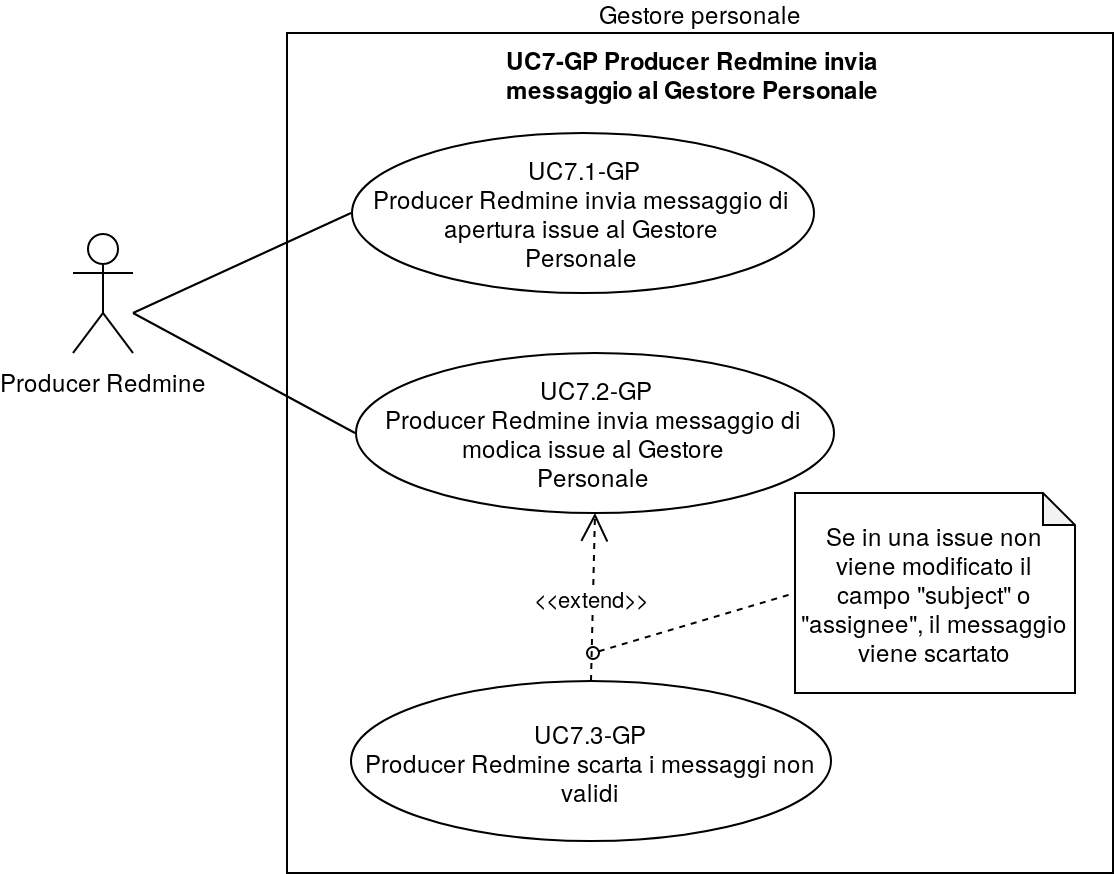
\includegraphics[width=0.7\textwidth]{img/casi_d'uso/UC7.png}\\
		\caption{UC\theuccount-GP - Producer GitLab invia messaggio al Gestore Personale}
	\end{figure}
	\begin{itemize}
		\item \textbf{Codice}: UC\theuccount-GP.
		\item \textbf{Titolo}: Producer GitLab invia messaggio al Gestore Personale.
		\item \textbf{Attori primari}: Producer GitLab.
		\item \textbf{Descrizione}: il Producer GitLab, dopo aver ricevuto una segnalazione da GitLab, elabora un messaggio da inviare al Gestore Personale.
		\item \textbf{Precondizione}: il Producer GitLab ha ricevuto una segnalazione da GitLab.
		\item \textbf{Postcondizione}: il Producer GitLab ha inviato al Gestore Personale il messaggio  \newline elaborato.
		\item \textbf{Scenario principale}: 
		\begin{enumerate}
			\item il Producer GitLab riceve una segnalazione da GitLab
			\item il Producer GitLab prepara il messaggio in modo che venga inserito correttamente nel Gestore Personale
			\item il Poducer GitLab invia il messaggio al Gestore Personale
		\end{enumerate}
		
	\end{itemize}
	\newpage
	\stepcounter{subuccount}
	\paragraph{UC\theuccount.\thesubuccount-GP - Producer GitLab invia uno o più messaggi di commit al Gestore Personale}
		
		\begin{itemize}
			\item \textbf{Codice}: UC\theuccount.\thesubuccount-GP.
			\item \textbf{Titolo}: Producer GitLab invia uno o più messaggi di commit al Gestore Personale.
			\item \textbf{Attori primari}: Producer GitLab.
			\item \textbf{Descrizione}: il Producer GitLab, dopo aver ricevuto una segnalazione di push da  \newline GitLab, elabora un messaggio particolare per i commit che verrà catalogato sotto il Topic "commits".
			Il messaggio elaborato conterrà i campi:
			\begin{itemize}
				\item Project
				\item Topic
				\item Message
			\end{itemize}
			\item \textbf{Precondizione}: il Producer GitLab ha ricevuto una segnalazione da GitLab.
			\item \textbf{Postcondizione}: il Producer GitLab ha inviato uno o più messaggi elaborati di commit.
			\item \textbf{Scenario principale}: 
			\begin{enumerate}
				\item Il Producer GitLab riceve la segnalazione di uno o più commit da GitLab
				\item Il Producer GitLab prepara i messaggi in modo che vengano inseriti correttamente nel Gestore Personale
				\item Il Poducer GitLab invia i messaggi di
				commit al Gestore Personale
			\end{enumerate}
			
		\end{itemize}
		
	\stepcounter{subuccount}
	\paragraph{UC\theuccount.\thesubuccount-GP -  Producer GitLab invia messaggio di issue al Gestore Personale}
		\begin{figure}[H]
			\centering
			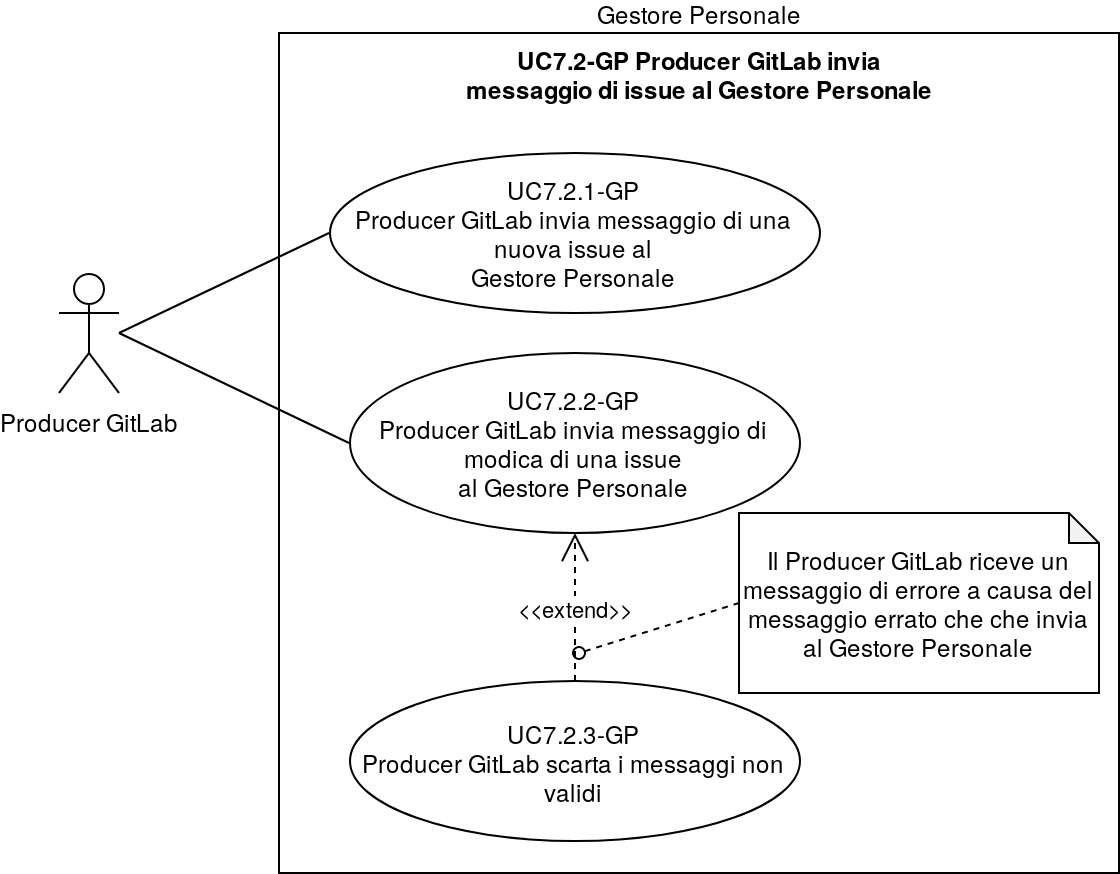
\includegraphics[width=0.8\textwidth]{img/casi_d'uso/UC7_2.png}\\
			\caption{UC\theuccount.\thesubuccount-GP -  Producer GitLab invia messaggio di issue al Gestore Personale}
		\end{figure}
		\begin{itemize}
			\newpage
			\item \textbf{Codice}: UC\theuccount.\thesubuccount-GP.
			\item \textbf{Titolo}:  Producer GitLab invia messaggio di issue al Gestore Personale.
			\item \textbf{Attori primari}: Producer GitLab.
			\item \textbf{Descrizione}: il Producer GitLab, dopo aver ricevuto una segnalazione di issue da GitLab, controlla se la issue è appena stata creata o si tratta della modifica di una issue preesistente. Il messaggio, una volta elaborato, conterrà i campi:
			\begin{itemize}
				\item Project
				\item Topic
				\item Subject e opzionalmente:
				\begin{itemize}
					\item Description
					\item Due Date
					\item Milestone
					\item Assignee
				\end{itemize}
			\end{itemize}
			\item \textbf{Precondizione}: il Producer GitLab ha ricevuto una segnalazione da GitLab.
			\item \textbf{Postcondizione}: il Producer GitLab ha inviato al Gestore Personale il messaggio  \newline elaborato.
			\item \textbf{Scenario principale}: 
			\begin{enumerate}
				\item Il Producer GitLab riceve la segnalazione di issue da GitLab
				\item Il Producer GitLab prepara il messaggio di issue in modo che venga inserito  \newline correttamente nel Gestore Personale
				\item Il Poducer GitLab invia il messaggio di issue al Gestore Personale
			\end{enumerate}
			
		\end{itemize}
		
		\stepcounter{subsubuccount}
		\subparagraph{UC\theuccount.\thesubuccount.\thesubsubuccount-GP - Producer GitLab invia messaggio di una nuova issue al Gestore Personale}
			
			\begin{itemize}
				\item \textbf{Codice}: UC\theuccount.\thesubuccount.\thesubsubuccount-GP.
				\item \textbf{Titolo}: Producer GitLab invia messaggio di una nuova issue al Gestore Personale.
				\item \textbf{Attori primari}: Producer GitLab.
				\item \textbf{Descrizione}: il Producer GitLab, dopo aver ricevuto una segnalazione di una nuova issue da GitLab, elabora il messaggio che conterrà i campi:
				\begin{itemize}
					\item Project
					\item Topic
					\item Subject e opzionalmente:
					\begin{itemize}
						\item Description
						\item Due Date
						\item Milestone
						\item Assignee
					\end{itemize}
				\end{itemize}
				\item \textbf{Precondizione}: il Producer GitLab ha ricevuto una segnalazione da GitLab.
				\item \textbf{Postcondizione}: il Producer GitLab ha inviato al Gestore Personale il messaggio   \newline elaborato di nuova issue.
				\item \textbf{Scenario principale}: 
				\begin{enumerate}
					\item Il Producer GitLab riceve la segnalazione di una nuova issue da GitLab
					\item Il Producer GitLab prepara il messaggio di una nuova issue in modo che venga inserito correttamente nel Gestore Personale
					\item Il Poducer GitLab invia il messaggio di una nuova issue al Gestore Personale
				\end{enumerate}
				
			\end{itemize}
		
		\stepcounter{subsubuccount}
		\subparagraph{UC\theuccount.\thesubuccount.\thesubsubuccount-GP - Producer GitLab invia messaggio di modifica di una issue al Gestore Personale}
			
			\begin{itemize}
				\item \textbf{Codice}: UC\theuccount.\thesubuccount.\thesubsubuccount-GP.
				\item \textbf{Titolo}: Producer GitLab invia messaggio di modifica di una issue al Gestore Personale.
				\item \textbf{Attori primari}: Producer GitLab.
				\item \textbf{Descrizione}: il Producer GitLab, dopo aver ricevuto una segnalazione di modifica di una issue da GitLab, controlla se sono stati modificati i campi Label o Title.
				In caso positivo, viene inviato un messaggio elaborato al Gestore Personale, il quale conterrà:
				\begin{itemize}
					\item Project
					\item Topic
					\item Subject e opzionalmente:
					\begin{itemize}
						\item Description
						\item Due Date
						\item Milestone
						\item Assignee
					\end{itemize}
				\end{itemize}
				\item \textbf{Precondizione}: il Producer GitLab ha ricevuto una segnalazione da GitLab.
				\item \textbf{Postcondizione}: il Producer GitLab ha inviato al Gestore Personale il messaggio   \newline elaborato di modifica issue.
				\item \textbf{Scenario principale}: 
				\begin{enumerate}
					\item Il Producer GitLab riceve la segnalazione di modifica issue da GitLab
					\item Il Producer GitLab prepara il messaggio di modifica issue in modo che venga inserito correttamente nel Gestore Personale
					\item Il Poducer GitLab invia il messaggio di modifica issue al Gestore Personale
				\end{enumerate}
				\item \textbf{Estensioni}: 
				\begin{enumerate}
					\item Se ci sono dei messaggi non validi, questi vengono scartati [UC\theuccount.\thesubuccount.3-GP].
				\end{enumerate}
			\end{itemize}
		
		\stepcounter{subsubuccount}
		\subparagraph{UC\theuccount.\thesubuccount.\thesubsubuccount-GP - Producer GitLab scarta i messaggi non validi}
			
			\begin{itemize}
				\item \textbf{Codice}: UC\theuccount.\thesubuccount.\thesubsubuccount-GP.
				\item \textbf{Titolo}: Producer GitLab scarta i messaggi non validi.
				\item \textbf{Attori primari}: Producer GitLab.
				\item \textbf{Descrizione}: il Producer GitLab, dopo aver ricevuto una segnalazione di una modifica issue da GitLab, controlla
				se sono stati modificati i campi Label o Title. In caso negativo, il messaggio viene scartato.
				\item \textbf{Precondizione}: il Producer GitLab ha ricevuto una segnalazione da GitLab.
				\item \textbf{Postcondizione}: il Producer GitLab ha scartato il messaggio.
				\item \textbf{Scenario principale}: 
				\begin{enumerate}
					\item Il Producer GitLab riceve la segnalazione di modifica issue da GitLab
					\item Il Producer GitLab vede che non sono stati modificati i campi Label o Title
					\item Il Producer GitLab scarta i messaggi non validi
				\end{enumerate}
			\end{itemize}